\documentclass[10pt]{beamer}
\usepackage[utf8]{inputenc}
\usepackage[russian]{babel}
\usepackage{graphicx, epsfig}
\usepackage{subfig}
\usepackage{floatflt}
\usepackage{epic,ecltree}
\usepackage{mathtext}
\usepackage{fancybox}
\usepackage{fancyhdr}
\usepackage{multirow}
\usepackage{enumerate}
\usepackage{epstopdf}
\usepackage{multicol}
\usepackage{algorithm}
\usepackage[noend]{algorithmic}
\def\algorithmicrequire{\textbf{Input:}}
\def\algorithmicensure{\textbf{Output:}}
\usetheme{Singapore}%{Singapore}%{Warsaw}%{Warsaw}%{Darmstadt}
\usecolortheme{default}
\setbeamertemplate{footline}[page number]{}
\setbeamerfont{title}{size=\Large}
\beamertemplatenavigationsymbolsempty

\setbeamersize{text margin left=3mm,text margin right=3mm} 

\usepackage{amsmath,amsfonts,amssymb,amsthm,mathtools} % AMS

\renewcommand{\epsilon}{\ensuremath{\varepsilon}}
\renewcommand{\phi}{\ensuremath{\varphi}}
\renewcommand{\kappa}{\ensuremath{\varkappa}}
\renewcommand{\le}{\ensuremath{\leqslant}}
\renewcommand{\leq}{\ensuremath{\leqslant}}
\renewcommand{\ge}{\ensuremath{\geqslant}}
\renewcommand{\geq}{\ensuremath{\geqslant}}
\renewcommand{\emptyset}{\varnothing}


\newcommand{\ba}{\mathbf{a}}
\newcommand{\bb}{\mathbf{b}}
\newcommand{\bc}{\mathbf{c}}
\newcommand{\be}{\mathbf{e}}
\newcommand{\bp}{\mathbf{p}}
\newcommand{\bq}{\mathbf{q}}
\newcommand{\bt}{\mathbf{t}}
\newcommand{\bu}{\mathbf{u}}
\newcommand{\bw}{\mathbf{w}}
\newcommand{\bx}{\mathbf{x}}
\newcommand{\by}{\mathbf{y}}
\newcommand{\bz}{\mathbf{z}}
\newcommand{\bA}{\mathbf{A}}
\newcommand{\bB}{\mathbf{B}}
\newcommand{\bC}{\mathbf{C}}
\newcommand{\bE}{\mathbf{E}}
\newcommand{\bF}{\mathbf{F}}
\newcommand{\bH}{\mathbf{H}}
\newcommand{\bJ}{\mathbf{J}}
\newcommand{\bP}{\mathbf{P}}
\newcommand{\bQ}{\mathbf{Q}}
\newcommand{\bR}{\mathbf{R}}
\newcommand{\bT}{\mathbf{T}}
\newcommand{\bU}{\mathbf{U}}
\newcommand{\bW}{\mathbf{W}}
\newcommand{\bX}{\mathbf{X}}
\newcommand{\bY}{\mathbf{Y}}

\newcommand{\bbR}{\mathbb{R}}
\newcommand{\bbX}{\mathbb{X}}
\newcommand{\bbY}{\mathbb{Y}}
\newcommand{\bbT}{\mathbb{T}}
\newcommand{\bbU}{\mathbb{U}}
\newcommand{\bbZ}{\mathbb{Z}}

\newcommand{\cA}{\mathcal{A}}
\newcommand{\cD}{\mathcal{D}}
\newcommand{\cL}{\mathcal{L}}

\newcommand{\bepsilon}{\boldsymbol{\varepsilon}}
\newcommand{\bchi}{\boldsymbol{\chi}}
\newcommand{\bnu}{\boldsymbol{\nu}}
\newcommand{\bmu}{\boldsymbol{\mu}}
\newcommand{\btheta}{\boldsymbol{\theta}}
\newcommand{\bTheta}{\boldsymbol{\Theta}}

\newcommand{\T}{^{\text{\tiny\sffamily\upshape\mdseries T}}}

\newcommand{\bOne}{\boldsymbol{1}}
\newcommand{\bZero}{\boldsymbol{0}}
\newcommand{\argmin}{\mathop{\arg \min}\limits}
\newcommand{\argmax}{\mathop{\arg \max}\limits}

\newcommand\undermat[2]{%
	\makebox[0pt][l]{$\smash{\underbrace{\phantom{%
					\begin{matrix}#2\end{matrix}}}_{\text{$#1$}}}$}#2}

\newtheorem{statement}{Утверждение}
\newtheorem{rustheorem}{Теорема}

% отображать название слайда слева
\setbeamertemplate{frametitle}[default][left]

%%% Рисунки
\usepackage{tikz}
\usetikzlibrary{matrix}

%\definecolor{beamer@blendedblue}{RGB}{15,120,80}
%----------------------------------------------------------------------------------------------------------
\title[\hbox to 56mm{  \hfill\insertframenumber\,/\,\inserttotalframenumber}]
{\\ \vspace{1.5cm} Снижение размерности пространства \\ в задачах декодирования сигналов}
\author[Роман Исаченко]{\\ 
	Исаченко Роман Владимирович \\
	\vspace{3mm}
	{\footnotesize 
	Диссертация на соискание ученой степени \\
	кандидата физико-математических наук
	} \\
	\vspace{0.2cm}
	{\footnotesize05.13.17 -- Теоретические основы информатики} \\
	\vspace{0.2cm}
	{\footnotesize Научный руководитель: д.ф.-м.н. В. В. Стрижов}
	}
\date{Москва, 2021 г.}
%--------------------------------------------------------------------------------
\begin{document}
%--------------------------------------------------------------------------------
\begin{frame}
%\thispagestyle{empty}
\titlepage
\end{frame}
%--------------------------------------------------------------------------------
\begin{frame}{Снижение размерности пространства в задачах декодирования сигналов}
	\begin{block}{Цель}
		Исследовать зависимости в пространствах объектов и ответов и построить устойчивую модель декодирования временных рядов в случае коррелированного описания объекта исследования.
	\end{block}
	\begin{block}{Проблема}
		Целевая переменная -- вектор, компоненты которого являются зависимыми. \\
		Требуется построить модель, адекватно описывающую как пространство объектов так и пространство ответов при наблюдаемой мультикорреляции в обоих пространствах высокой размерности. 
	\end{block}
	\begin{block}{Решение}
		Для учёта зависимостей в пространствах объектов и ответов предлагается снизить размерность, используя скрытое пространство. Предлагаются линейные и нейросетевые методы согласования связанных моделей в пространствах высокой размерности.
	\end{block}
\end{frame}
%--------------------------------------------------------------------------------
\begin{frame}{Задача декодирования сигналов}
    \begin{figure}
    	\includegraphics[width=0.85\linewidth]{figs/slide3_1}
    \end{figure}

	\begin{minipage}{.45\linewidth}
		\vspace{-0.2cm}
		\begin{block}{Авторегрессионная модель}
		\begin{figure}
			\includegraphics[width=\linewidth]{figs/slide3_3}
		\end{figure}
		\end{block}
		
	\end{minipage}%
	\begin{minipage}{.55\linewidth}
		\begin{block}{Проекция в скрытое пространство}
			\begin{figure}
				\includegraphics[width=0.75\linewidth]{figs/slide3_2}
			\end{figure}
			\vspace{-0.4cm}
			\begin{align*}
				\bX &= \bT \bP^{\T} + \bE_{\bx} \\
				\bY &= \bU \bQ^{\T} + \bE_{\by} \\
			\end{align*}
		\vspace{-1.0cm}
		\[
			\text{cov} (\bT, \bU) \rightarrow \max_{\bP, \bQ}
		\]
		\end{block}
	\vspace{0.3cm}
	\end{minipage}

\end{frame}
%--------------------------------------------------------------------------------
\begin{frame}{Задача авторегрессионного прогнозирования}
	$\bX = [\bchi_1, \dots, \bchi_n] \in \bbR^{m \times n}$~-- матрица объектов; \\
	$\bY = [\bnu_1, \dots, \bnu_r] \in \bbR^{m \times r}$~-- матрица ответов; \\
	$\by = \bTheta \bx+ \boldsymbol{\varepsilon}, \quad \bTheta \in \bbR^{r \times n}$~-- модель.
\begin{block}{Функция потерь линейной модели декодирования}
	\vspace{-0.4cm}
	\[
	\mathcal{L}(\bTheta | \bX, \bY) = {\left\| \underset{m \times r}{\mathbf{Y}}  - \underset{m \times n}{\bX} \cdot \underset{r \times n}{\bTheta}^{\T} \right\| }_2^2 \rightarrow\min_{\bTheta}; \quad 
	\bTheta^{\T} = (\bX^{\T} \bX)^{-1} \bX^{\T} \bY.
	\]
\end{block}
Для устранения сильной линейной зависимости столбцов матрицы~$\bX$ предлагается использовать методы снижения размерности пространства. 
\begin{block}{Метод проекции в скрытое пространство}
	\vspace{-0.7cm}
	\begin{align*}
		\underset{m \times n}{\vphantom{\bQ}\bX} 
		&= \underset{m \times l}{\vphantom{\bQ}\bT} \cdot \underset{l \times n}{\vphantom{\bQ}\bP^{\T}} + \underset{m \times n}{\vphantom{\bQ}\bE_{\bx}} 
		= \sum_{k=1}^l \underset{m \times 1}{\vphantom{\bp_k^{\T}}\bt_k} \cdot \underset{1 \times n}{\bp_k^{\T}} + \underset{m \times n}{\vphantom{\bp_k^{\T}}\bE_{\bx}},\\
		\underset{m \times r}{\vphantom{\bQ}\bY} 
		&= \underset{m \times l}{\vphantom{\bQ}\bU} \cdot \underset{l \times r}{\bQ^{\T}} + \underset{m \times r}{\vphantom{\bQ}\bE_{\by}}
		=  \sum_{k=1}^l  \underset{m \times 1}{\vphantom{\bq_k^{\T}}\bu_k} \cdot \underset{1 \times r}{\bq_k^{\T}} +  \underset{m \times r}{\vphantom{\bq_k^{\T}}\bE_{\by}}.
	\end{align*}
	\vspace{-0.2cm}
	\begin{equation*}
		\hat{\bY} = f(\bX) = \bX \bTheta; \quad \bU \approx \bT \bB, \quad \bB = \text{diag}(\beta_k), \quad \beta_k = \bu_k^{\T}\bt_k / (\bt_k^{\T}\bt_k).
	\end{equation*}
	\vspace{-0.2cm}
\end{block}

\end{frame}
%--------------------------------------------------------------------------------
\begin{frame}{Пример проекции в скрытое пространство в двумерном случае}
	\begin{itemize}
		\item $\bx_i \sim \mathcal{N}(0, \mathbf{\Sigma})$;
		\item $\by_i$ линейно зависят от $pc_2$ и не зависят от $pc_1$.
	\end{itemize}	
	\begin{figure}[h]
	\centering
	\includegraphics[width=\linewidth]{figs/pls_toy_example}
	\end{figure}
	Учёт взаимной корреляции между проекциями матриц~$\bX$ и~$\bY$ отклоняет вектора~$\bw_k$ и~$\bc_k$ от направления главных компонент. 
\end{frame}
%--------------------------------------------------------------------------------
\begin{frame}{Метод проекции в скрытое пространство}

\begin{statement}[Исаченко, 2017]
	Максимизация ковариации между векторами~$\bt_k$ и $\bu_k$ приводит к наилучшему описанию матриц $\bX$ и $\bY$ с учётом их взаимосвязи.
\end{statement}
\begin{statement}[Исаченко, 2017]
	Вектора $\bw_k$ и $\bc_k$~-- собственные вектора матриц~$\bX_k^{\T} \bY_k \bY_k^{\T} \bX_k$ и $\bY_k^{\T} \bX_k \bX_k^{\T} \bY_k$, соответствуюшие максимальным собственным значениям.
\end{statement}
\begin{statement}[Исаченко, 2017]
	Правила обновления векторов максимизируют ковариацию между векторами~$\bt_k$ и $\bu_k$.
\end{statement}

\begin{block}{Модель проекции в скрытое пространство}
	
	\[
	\bY = \bU \bQ^{\T} + \bE_{\by} \approx \bT \bB \bQ^{\T}+ \bE_{\by} = \bX \bW^* \bB \bQ^{\T} + \bE = \bX \bTheta + \bE_{\by}.
	\]
	\[
	\bTheta = \bW (\bP^{\T} \bW)^{-1} \bB \bQ^{\T}, \quad \bT = \bX \bW^*, \quad \text{where } \bW^* = \bW (\bP^{\T} \bW)^{-1}.
	\]
\end{block}
\end{frame}
%--------------------------------------------------------------------------------
\begin{frame}{Скрытое пространство в задаче декодирования}
	
	\textbf{Особенностью задачи} является избыточность описания переменных $\bx$ и $\by$.
	Объекты $\bx$ и $\by$ живут на некоторых многообразиях низкой размерности. 
	\begin{figure}
		\includegraphics[width=0.32\linewidth]{figs/decoding_scheme}
	\end{figure}
		
	Пространства $\bbT \subset \bbR^l$ и $\bbU \subset \bbR^s$ \textit{скрытые пространства} для $\bbX \in \bbR^n$ ($l \leq n$) и $\bbY \in \bbR^r (s \leq r)$, если существуют \textit{функции кодировании} $\varphi_e: \bbX \to \bbT$, $\psi_e: \bbY \to \bbU$ и \textit{функции декодирования} $\varphi_d: \bbT  \to \bbX$, $\psi_d: \bbU  \to \bbY$:
	\begin{align*}
	\text{для любого } \bx \in \bbX &\quad \text{существует } \bt \in \bbT: \varphi_d (\varphi_e(\bx)) = \varphi_d(\bt) = \bx; \\
	\text{для любого } \by \in \bbY &\quad  \text{существует } \bu \in \bbU: \psi_d (\psi_e(\by)) = \psi_d(\bu) = \by.
	\end{align*}
	Cкрытыe пространства $\bbT$ и $\bbU$ являются \textit{согласованными}, если существует \textit{функция согласования} $h: \bbT \rightarrow \bbU$:
	\[
		\by = f(\bx) = \psi_d(h(\phi_e(x))).
	 \]
	
\end{frame}
%--------------------------------------------------------------------------------
\begin{frame}{Выбор признаков в задаче декодирования}
\begin{block}{Требуется}
Найти бинарный вектор~$\ba = \{0, 1\}^n$, компоненты~-- индикаторы выбранных признаков. 
\end{block}
\begin{block}{Функция ошибки отбора признаков}
	\vspace{-0.2cm}
\[
\ba = \argmin_{\ba' \in \{0, 1\}^n} S(\ba' | \bX, \bY).
\]
\vspace{-0.5cm}
\end{block}
\begin{block}{Релаксация}
	Замена дикретной области определения $\{0, 1\}^n$ на непрерывную релаксацию $[0, 1]^n$:
	\[
	\bz = \argmin_{\bz' \in [0, 1]^n} S(\bz' | \bX, \bY), \quad 
	a_j = [z_j > \tau].
\]
\end{block}
Получив~$\ba$, решаем задачу регрессии:
\[
\mathcal{L}(\bTheta_{\ba} | \bX_{\ba}, \bY) = {\left\| \mathbf{Y} - \bX_{\ba}\bTheta^{\T}_{\ba} \right\| }_2^2 \rightarrow\min_{\bTheta_{\ba}},
\]
где индекс~$\ba$ обозначает подматрицу с номерами столбцов, для которых~$a_j = 1$.
\end{frame}
%--------------------------------------------------------------------------------
\begin{frame}{Выбор признаков с помощью квадратичного программирования}
	\[
	\| \bnu - \bX \btheta\|_2^2 \rightarrow\min_{\btheta \in \bbR^{n}}.
	\]
	\vspace{-0.3cm}
	\begin{block}{Задача квадратичного программирования}
	\vspace{-0.3cm}
	\[
	S(\bz | \bX, \bnu)	= (1 - \alpha) \cdot \underbrace{\bz^{\T} \bQ \bz}_{\text{Sim}(\bX)} - \alpha \cdot \underbrace{\vphantom{()} \mathbf{b}^{\T} \bz}_{\text{Rel}(\bX, \bnu)} \rightarrow \min_{\substack{\bz \geq \bZero_n \\ \bOne_n^{\T} \bz=1}}.
	\]
	\vspace{-0.3cm}
	\end{block}
		$\bz \in [0, 1]^n$ -- значимость признаков; \\
		$\bQ \in \bbR^{n \times n}$ -- матрица парных взаимодействий признаков; \\
		$\mathbf{b} \in \bbR^n$ -- вектор релевантностей признаков к целевой переменной.
		\[
		\bQ = \bigl[\left|\text{corr}(\bchi_i, \bchi_j)\right|\bigr]_{i,j=1}^n, \quad
		\bb = \bigl[\left|\text{corr}(\bchi_i, \bnu)\right|\bigr]_{i=1}^n.
		\]
\vspace{-0.2cm}
\begin{statement}[Исаченко, 2018]
	В случае полуопределенной матрицы~$\bQ$ задача QPFS является выпуклой. 
	Полуопределенная релаксация~-- сдвиг спектра:
\end{statement}
\vspace{-0.3cm}
\begin{equation*}
\bQ \rightarrow \bQ - \lambda_{\min} \mathbf{I}.
\end{equation*}
\end{frame}
%--------------------------------------------------------------------------------
\begin{frame}{Многомерный выбор признаков в задаче декодирования}
\begin{block}{Агрегирование релевантностей по целевым векторам (RelAgg)}
\[
\bb = \left[\left|\text{corr}(\bchi_i, \bnu)\right|\right]_{i=1}^n \rightarrow \bb = \left[\sum_{k=1}^r\left|\text{corr}(\bchi_i, \bnu_k)\right|\right]_{i=1}^n.
\]
\end{block}
{\bf Недостаток:} нет учёта зависимостей в матрице~$\bY$. 

\begin{block}{Симметричный учёт значимостей (SymImp)}
Штрафуем коррелированные целевые вектора с помощью~$\text{Sim} (\bY)$
\[
\alpha_1 \cdot \underbrace{\bz_x^{\T} \bQ_x \bz_x}_{\text{Sim}(\bX)} - \alpha_2 \cdot \underbrace{\bz_x^{\T} \bB \bz_y}_{\text{Rel}(\bX, \bY)} + \alpha_3 \cdot \underbrace{\bz_y^{\T} \bQ_y \bz_y}_{\text{Sim}(\bY)} \rightarrow \min_{\substack{\bz_x \geq \bZero_n, \, \bOne_n^{\T}\bz_x=1 \\ \bz_y \geq \bZero_r, \, \bOne_r^{\T}\bz_y=1}}.
\]
\[
\bQ_x = \left[ \left| \text{corr}(\bchi_i, \bchi_j) \right| \right]_{i,j=1}^n, \,
\bQ_y = \left[ \left| \text{corr}(\bnu_i, \bnu_j) \right| \right]_{i,j=1}^r, \,
\bB =  \left[ \left| \text{corr}(\bchi_i, \bnu_j) \right| \right]_{\substack{i=1, \dots, n \\ j=1, \dots, r}}.
\]
\[
\alpha_1 + \alpha_2 + \alpha_3 = 1, \quad \alpha_i \geq 0.
\] 
\end{block}
\end{frame}
%--------------------------------------------------------------------------------
\begin{frame}{Многомерный выбор признаков в задаче декодирования}
	SymImp штрафует коррелированные целевые вектора, которые в меньшей мере объясняются признаками. 
	\[
	\alpha_1 \cdot \underbrace{\bz_x^{\T} \bQ_x \bz_x}_{\text{Sim}(\bX)} - \alpha_2 \cdot \underbrace{\vphantom{()} \bz_x^{\T}\mathbf{B} \bz_y}_{\text{Rel}(\bX, \bY)} \rightarrow \min_{\substack{\bz_x \geq \bZero_n \\ \bOne_n^{\T}\bz_x=1}}; \quad
	\alpha_3 \cdot \underbrace{\bz_y^{\T} \bQ_y \bz_y}_{\text{Sim}(\bY)} + \alpha_2 \cdot \underbrace{\vphantom{()} \bz_x^{\T} \mathbf{B} \bz_y}_{\text{Rel}(\bX, \bY)} \rightarrow \min_{\substack{\bz_y \geq \bZero_r  \\ \bOne_r^{\T}\bz_y=1}}.
	\]
	\vspace{-0.2cm}
	\begin{block}{Минимаксный подход (MinMax / MaxMin)}
	\vspace{-0.5cm}
	\[
	\min_{\substack{\bz_x \geq \bZero_n \\ \bOne_n^{\T}\bz_x=1}} 	\max_{\substack{\bz_y \geq \bZero_r \\ \bOne_r^{\T}\bz_y=1}} \Bigl(\text {or} \, \max_{\substack{\bz_y \geq \bZero_r \\ \bOne_r^{\T}\bz_y=1}} \min_{\substack{\bz_x \geq \bZero_n \\ \bOne_n^{\T}\bz_x=1}}\Bigr) \Bigl[\alpha_1 \cdot \underbrace{\bz_x^{\T} \bQ_x \bz_x}_{\text{Sim}(\bX)} - \alpha_2 \cdot \underbrace{\bz_x^{\T} \bB \bz_y}_{\text{Rel}(\bX, \bY)} - \alpha_3 \cdot \underbrace{\bz_y^{\T} \bQ_y \bz_y}_{\text{Sim}(\bY)}\Bigr].
	\]
	\end{block}
	\vspace{-0.4cm}
	\begin{rustheorem}[Исаченко, 2018]
		Для положительно определенных матриц $\bQ_x$ и $\bQ_y$ minmax и maxmin задачи достигают одинакового значения функционала.
	\end{rustheorem}
	\vspace{-0.2cm}
	\begin{rustheorem}[Исаченко, 2018]
		Минимаксная задача эквивалентна задаче квадратичного программирования с $n + r + 1$ переменными.
	\end{rustheorem}
	Для получения выпуклой задачи применяется сдвиг спектра.

\end{frame}
%--------------------------------------------------------------------------------
\begin{frame}{Многомерный выбор признаков в задаче декодирования}
	\begin{block}{Максимизация релевантностей (MaxRel)}
	\vspace{-0.2cm}
	\[
		\min_{\substack{\bz_x \geq \bZero_n \\ \bOne_n^{\T}\bz_x=1}} 	\max_{\substack{\bz_y \geq \bZero_r \\ \bOne_r^{\T}\bz_y=1}} \left[ (1 - \alpha) \cdot \bz_x^{\T} \bQ_x \bz_x - \alpha \cdot \bz_x^{\T} \bB \bz_y \right].
	\]
	\vspace{-0.2cm}
	\end{block}
	\begin{rustheorem}[Исаченко, 2018]
		Для положительно определенной матрицы $\bQ_x$ minmax и maxmin задачи достигают одинакового значения функционала.
	\end{rustheorem}
	\begin{block}{Асимметричный учёт значимостей (AsymImp)}
	\vspace{-0.2cm}
	\begin{equation*}
	\alpha_1 \cdot \underbrace{\bz_x^{\T} \bQ_x \bz_x}_{\text{Sim}(\bX)} - \alpha_2 \cdot  \underbrace{\left(\bz_x^{\T} \bB \bz_y - \bb^{\T} \bz_y \right) }_{\text{Rel}(\bX, \bY)} + \alpha_3 \cdot \underbrace{\bz_y^{\T} \bQ_y \bz_y}_{\text{Sim}(\bY)} \rightarrow \min_{\substack{\bz_x \geq \bZero_n, \, \bOne_n^{\T}\bz_x=1 \\ \bz_y \geq \bZero_r, \, \bOne_r^{\T}\bz_y=1}}.
	\end{equation*}
	\vspace{-0.4cm} \\
	При $b_j = \max\limits_{i=1, \dots n} [\bB]_{i, j}$ коэффициенты при~$\bz_y$ в~$\text{Rel}(\bX, \bY)$ неотрицательны.
	
	\begin{statement}[Исаченко, 2017]
		В одномерном случае $r=1$ предлагаемые стратегии SymImp, MinMax, MaxMin, MaxRel, AsymImp совпадают с исходным алгоритмом QPFS.
	\end{statement}
\end{block}
\end{frame}
%--------------------------------------------------------------------------------
\begin{frame}{Обобщение предложенных методов выбора признаков}
\begin{table}
	\centering
	\footnotesize{
		\begin{tabular}{c|c|c}
			\hline
			Алгоритм & Критерий & Функция ошибки $S(\bz | \bX, \bY)$ \\
			\hline && \\ 
			RelAgg & $\min \bigl[ \text{Sim}(\bX) - \text{Rel}(\bX, \bY) \bigr] $ & $\min\limits_{\bz_x} \bigl[ (1 - \alpha) \cdot \bz_x^{\T} \bQ_x \bz_x - \alpha \cdot \bz_x^{\T} \bB \bOne_r \bigr] $ \\ &&\\
			SymImp & $\begin{aligned} \min \, \bigl[ \text{Sim}(\bX) & - \text{Rel}(\bX, \bY) \\ & + \text{Sim}(\bY) \bigr] \end{aligned}$ & $ \min\limits_{\bz_x, \, \bz_y} \left[ \alpha_1 \cdot \bz_x^{\T} \bQ_x \bz_x - \alpha_2 \cdot \bz_x^{\T} \bB \bz_y + \alpha_3 \cdot \bz_y^{\T} \bQ_y \bz_y \right] $\\ &&\\ 
			MinMax & $\begin{aligned} &\min \, \bigl[ \text{Sim}(\bX) - \text{Rel}(\bX, \bY) \bigr]  \\ & \max \bigl[\text{Rel}(\bX, \bY) + \text{Sim}(\bY) \bigr] \end{aligned}$ & $	\min\limits_{\bz_x} 	\max\limits_{\bz_y} \bigl[\alpha_1 \cdot \bz_x^{\T} \bQ_x \bz_x - \alpha_2 \cdot \bz_x^{\T} \bB \bz_y - \alpha_3 \cdot \bz_y^{\T} \bQ_y \bz_y \bigr]$ \\ &&\\ 
			MaxRel & $\begin{aligned} &\min \, \bigl[ \text{Sim}(\bX) - \text{Rel}(\bX, \bY) \bigr]  \\ & \max \bigl[\text{Rel}(\bX, \bY) \bigr] \end{aligned}$& $\min\limits_{\bz_x} 	\max\limits_{\bz_y} \bigl[ (1 - \alpha) \cdot \bz_x^{\T} \bQ_x \bz_x - \alpha \cdot \bz_x^{\T} \bB \bz_y \bigr]$ \\ 		&&\\
			AsymImp & $\begin{aligned} & \min \, \bigl[ \text{Sim}(\bX) - \text{Rel}(\bX, \bY) \bigr]\\ &  \max \bigl[\text{Rel}(\bX, \bY) + \text{Sim}(\bY) \bigr] \end{aligned}$ & $\min\limits_{\bz_x, \bz_y} \bigl[ \alpha_1 \bz_x^{\T} \bQ_x \bz_x - \alpha_2 \left(\bz_x^{\T} \bB \bz_y - \bb^{\T} \bz_y \right) + \alpha_3  \bz_y^{\T} \bQ_y \bz_y \bigr]$\\  && \\
			\hline
	\end{tabular}}
\end{table}
\end{frame}
%--------------------------------------------------------------------------------
\begin{frame}{Внешние критерии качества решения задачи декодирования}

\begin{block}{Нормированное RMSE}
	Качество предсказания:
	\vspace{-0.2cm}
	\[
		\text{sRMSE}(\bY, \widehat{\bY}_{\ba}) = \sqrt{\frac{\text{MSE} (\bY, \widehat{\bY}_{\ba})}{\text{MSE} (\bY, \overline{\bY})}} =  \frac{\| \bY - \widehat{\bY}_{\ba} \|_2}{\| \bY - \overline{\bY} \|_2}, \quad \text{где} \quad \widehat{\bY}_{\ba} = \bX_{\ba} \bTheta_{\ba}^{\T}.
	\]
	\vspace{-0.2cm}
	$\overline{\bY}$~--- константный прогноз.
\end{block}

\begin{block}{Мультикорреляция}
	Среднее значение коэффициента множественной корреляции:
	\vspace{-0.2cm}
	\[
		R^2 = \frac{1}{r} \text{tr} \left( \bC^{\T} \mathbf{R}^{-1} \bC \right); \quad \bC = [ \text{corr}(\bchi_i, \bnu_j)]_{\substack{i=1, \dots, n \\ j=1, \dots, r}}, \, \mathbf{R} = [ \text{corr}(\bchi_i, \bchi_j)]_{i, j = 1}^n.
	\]
\end{block}
\vspace{-0.4cm}
\begin{block}{BIC}
	Компромисс между качеством предсказания и числом выбранных признаков~$\|\ba\|_0$:
	\vspace{-0.3cm}
	\[
		\text{BIC} = m \ln \left( \text{MSE} ( \bY, \widehat{\bY}_{\ba})\right) + \| \ba \|_0 \cdot \log m.
	\]
\end{block}
\end{frame}
%--------------------------------------------------------------------------------
\begin{frame}{Задача восстановления траектории конечности по сигналам электрокортикограммы}
    \begin{figure}
    	\includegraphics[width=0.85\linewidth]{figs/slide3_1}
    \end{figure}
	\begin{minipage}{.55\linewidth}
	\begin{itemize}
		\item $\bX \in \bbR^{m \times (32 \cdot 27)}$ -- сигналы ECoG.
		\item $\bY \in \bbR^{m \times 3k}$ -- траектория движения руки.
	\end{itemize}
	\vspace{0.1cm}
	\[
		\bY = 
		\begin{pmatrix}
		x_1 \,\, y_1 \,\, z_1 & \dots & x_{k\hphantom{+1}} \,\, y_{k\hphantom{+1}} \,\, z_{k\hphantom{+1}}\\
		x_2 \,\, y_2 \,\, z_2 & \dots & x_{k + 1} \,\, y_{k + 1} \,\, z_{k + 1}\\
		 \dots & \dots & \dots  \\
		x_m \, y_m \, z_m & \dots & x_{m + k} \, y_{m + k} \, z_{m + k}
		\end{pmatrix}
	\]
	\end{minipage}%
	\begin{minipage}{.43\linewidth}
		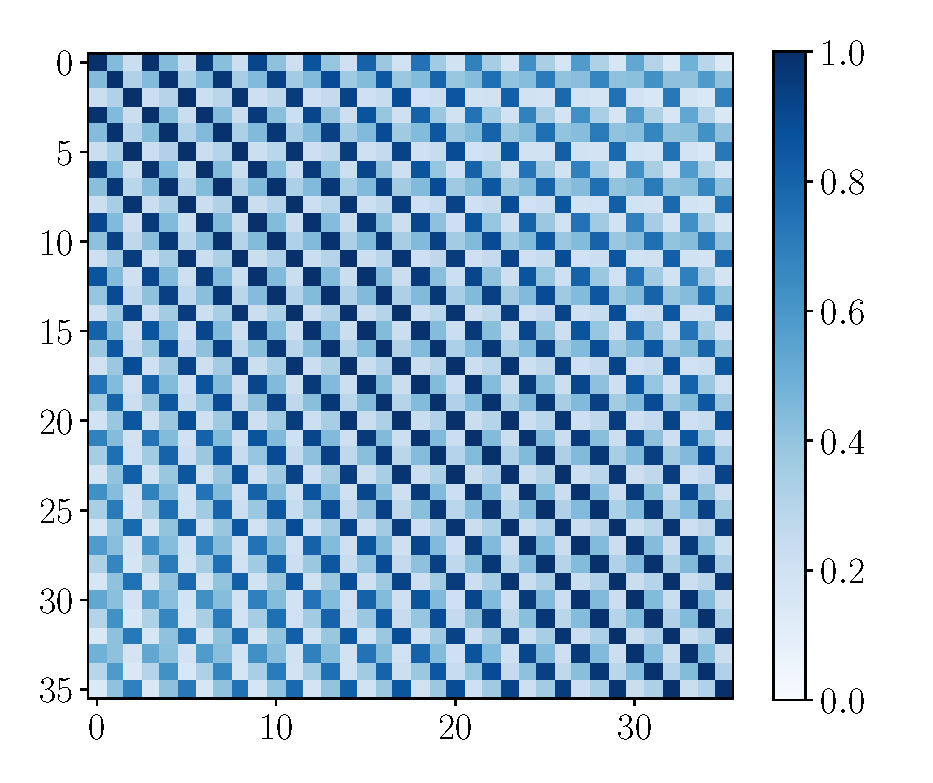
\includegraphics[width=0.9\linewidth]{figs/Y_corr_matrix.eps}
		\begin{center}
			\vspace{-0.4cm}
			Матрица корреляций $\bY$
			\vspace{-0.4cm}
		\end{center}
	\end{minipage}
	\\
	\url{http://neurotycho.org}
\end{frame}
%--------------------------------------------------------------------------------
\begin{frame}{Анализ предложенных методов выбора признаков}
	\begin{figure}
		\includegraphics[width=0.85\linewidth]{figs/ecog_3_30_metrics.pdf}
	\end{figure}
	Предложенные методы выбирают модель с меньшей ошибкой по отношению к базовому алгоритму.
\end{frame}

%--------------------------------------------------------------------------------
\begin{frame}{Стабильность методов выбора признаков}
\begin{block}{Постановка эксперимента}
	\begin{itemize}
	\item cоздать бутстреп-выборки
	\vspace{-0.1cm}
	\[
		(\bX, \bY) \rightarrow \bigl\{(\bX_1, \bY_1), \dots, (\bX_s, \bY_s)\bigr\};
	\]
	\item решить задачу выбора признаков
	\vspace{-0.1cm}
	\[
		 \bigl\{(\bX_1, \bY_1), \dots, (\bX_s, \bY_s)\bigr\}  \rightarrow \{\bz_1, \dots, \bz_s\};
	\]
	\item вычислить статистики
	\vspace{-0.1cm}
	\end{itemize}
	\[
		\{\bz_1, \dots, \bz_s\} \rightarrow \{ \text{sRMSE}, \|\ba\|_0, \text{Спирмен }\rho, \ell_2 \text{ расстояние}\}.
	\]
\end{block}
\renewcommand{\arraystretch}{1.2}
\begin{table}[]
	\centering
	\begin{tabular}{l|ccccc}
		\hline
		& sRMSE  & $\|\ba\|_0$ & Спирмен $\rho$ & $\ell_2$ расстояние \\ \hline
		RelAgg & 0.965 $\pm$ 0.002 & 26.8 $\pm$ 3.8 & 0.915 $\pm$ 0.016 & 0.145 $\pm$ 0.018   \\
		SymImp & 0.961 $\pm$ 0.001 & 224.4 $\pm$ 9.0 & 0.910 $\pm$ 0.017 & 0.025 $\pm$ 0.002   \\
		MinMax & 0.961 $\pm$ 0.002 & 101.0 $\pm$ 2.1& 0.932 $\pm$ 0.009 & 0.059 $\pm$ 0.004   \\
		MaxRel & 0.958 $\pm$ 0.003 & 41.2 $\pm$ 5.2 & 0.862 $\pm$ 0.027 & 0.178 $\pm$ 0.010   \\
		AsymImp & 0.955 $\pm$ 0.001 & 85.8 $\pm$ 10.2& 0.926 $\pm$ 0.011 & 0.078 $\pm$ 0.007  \\ \hline
	\end{tabular}
\end{table}
\end{frame}
%--------------------------------------------------------------------------------
\begin{frame}{Сравнение метода проекции в скрытое пространство с методами выбора признаков}

\begin{figure}[h]
	\begin{minipage}{.43\linewidth}
		\centering
		\includegraphics[width=1.\linewidth]{figs/pls_vs_k}
	\end{minipage}%
	\begin{minipage}{.57\linewidth}
		\centering
		\includegraphics[width=1.\linewidth]{figs/models2}
	\end{minipage}
\end{figure}
\begin{itemize}
	\item Предлагаемые методы выбора признаков достигают меньшей ошибки по сравнению с базовыми алгоритмами Lasso и Elastic.
	\item PLS показывает сравнимое качество с QPFS.
	\item Комбинация двух алгоритмов показывает наилучший результат.
\end{itemize}

\end{frame}
%--------------------------------------------------------------------------------
\begin{frame}{Нелинейные методы согласования скрытого пространства}
	
	\begin{minipage}{.65\linewidth}
		\begin{block}{Нелинейная проекция в скрытое пространство}
			\vspace{-0.3cm}
			\begin{align*}
				\bT &= \varphi_e(\bX) =  \bW_x^L \sigma(\dots \sigma(\bW_x^2 \sigma(\bX \bW_x^1)) \dots ) \\
				\bU &= \psi_e(\bY) =  \bW_y^L \sigma(\dots \sigma(\bW_y^2 \sigma(\bY \bW_y^1)) \dots ) \\
				\bX &= \varphi_d(\bX) =  \bW_t^L \sigma(\dots \sigma(\bW_x^2 \sigma(\bT \bW_t^1)) \dots ) \\
				\bY &= \psi_d(\bY) =  \bW_u^L \sigma(\dots \sigma(\bW_y^2 \sigma(\bU \bW_u^1)) \dots )
			\end{align*}
			\vspace{-0.3cm}
		\end{block}
		\begin{block}{Согласование проекций}
		\[
		g(\bT, \bU) \rightarrow \max_{\bW},
		\]
		где $\bW = \{\{\bW_x^i\}_{i=1}^L, \{\bW_y^i\}_{i=1}^L, \{\bW_t^i\}_{i=1}^L, \{\bW_u^i\}_{i=1}^L\}$.
		\end{block}	
	\end{minipage}%
	\begin{minipage}{.35\linewidth}
		\begin{figure}
			\includegraphics[width=1.0\linewidth]{figs/decoding_scheme}
		\end{figure}
	\begin{block}{Данные рукописных цифр}
		\begin{figure}
			\includegraphics[width=1.0\linewidth]{figs/left_right_mnist}
		\end{figure}
	\end{block}
	
	\end{minipage}

\end{frame}
%--------------------------------------------------------------------------------
\begin{frame}{Результаты, выносимые на защиту}
\begin{enumerate}
	\item Исследована задача декодирования сигналов в пространствах высокой размерности. Исследованы методы снижения размерности с анализом структуры пространства.
	\vfill
	\item Доказаны теоремы об оптимальности предлагаемых методов декодирования сигналов.
	\vfill 
	\item Предложены методы для выбора признаков, учитывающие зависимости как в пространстве объектов, так и в пространстве ответов. Предложенные алгоритмы доставляют устойчивые и адекватные решения в коррелированных пространствах высокой размерности.
	\vfill
	\item Предложены нелинейные методы согласования скрытых пространств для данных со сложно организованной целевой переменной.
	\vfill
	\item Создан макет системы решения задачи декодирования сигналов в пространствах высокой размерности.
\end{enumerate}
\end{frame}
%--------------------------------------------------------------------------------
\begin{frame}{Заключение}
	\begin{block}{Публикации ВАК}
		{\scriptsize
		\begin{enumerate}
			\item Isachenko R., Strijov V. Quadratic Programming Feature Selection for Multicorrelated Signal Decoding with Partial Least Squares \emph{Expert Systems with Applications}, 2021, на рецензировании.
			\item Исаченко Р.В., Яушев Ф.Р., Стрижов В.В. Модели согласования скрытого пространства в задаче прогнозирования // Системы и средства информатики, 31(1), 2021.
			\item Isachenko~R., Vladimirova~M., Strijov~V. Dimensionality Reduction for Time Series Decoding and Forecasting Problems. \emph{DEStech Transactions on Computer Science and Engineering}, optim, 2018.
			\item Isachenko~R., Strijov~V. Quadratic programming optimization for Newton method. \emph{Lobachevskii Journal of Mathematics}, 39(9), 2018.
			\item Isachenko~R. et al. Feature Generation for Physical Activity Classification. \emph{Artificial Intellegence and Decision Making}, 3, 2018.
			\item Исаченко Р.В., Стрижов В. В. Метрическое обучение в задачах мультиклассовой классификации временных рядов \emph{Информатика и её применения}, 10(2), 2016.
		\end{enumerate}
	}
	\end{block}
\vspace{-0.2cm}
\begin{block}{Выступления с докладом}
	{\scriptsize
	\begin{enumerate}
		\item  Intelligent Data Processing Conference, 2020, Снижение размерности в задаче декодирования временных рядов.
		\item  Intelligent Data Processing Conference, 2018, Dimensionality reduction for multicorrelated signal decoding with projections to latent space. 
		\item Математические методы распознавания образов, 2017. Локальные модели для классификации объектов сложной структуры.
		\item Intelligent Data Processing Conference, 2016. Multimodel forecasting multiscale time series in internet of things.
		\item Ломоносов, 2016. Метрическое обучение в задачах мультиклассовой классификации временных рядов.
	\end{enumerate}
	}
\end{block}
\end{frame}
\end{document} 
